\chapter{预备知识}

\label{sec:background}
在本章中,将介绍普通和加密重复数据删除方法的基础知识,以及加密重复数据删除仍然容易受到攻击的原因。

\section{重复数据删除}

\begin{figure}[!htb]
    \small
    \centering
    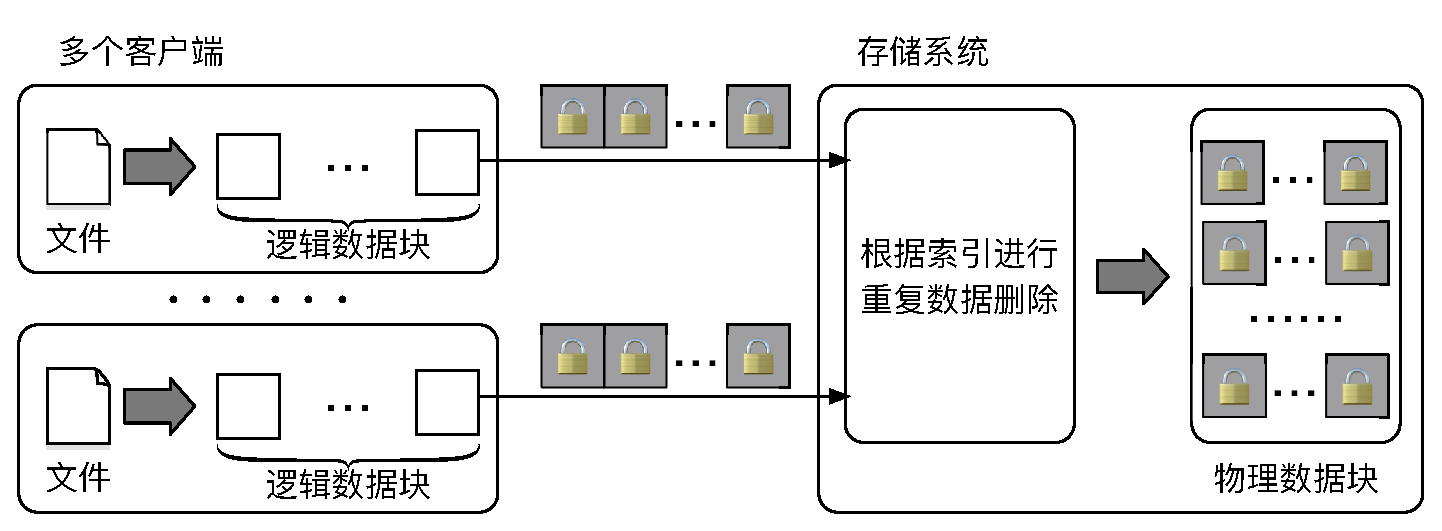
\includegraphics[width=14cm]{DedupSystemView.eps}
    \caption{重复数据删除的工作流程概览} 
    \label{fig:重复数据删除的工作流程概览}
\end{figure}

本文专注于基于块的重复数据删除,它以称为数据块的小型数据单元为粒度运行。图\ref{fig:重复数据删除的工作流程概览}总结了重复数据删除工作流程。 

具体地,重复数据删除系统首先通过文件切块过程将客户端的文件(例如,备份文件)分割成逻辑数据块,根据每一个逻辑数据块的内容使用HASH算法(哈希算法)计算得到其对应的唯一标签(又成为指纹)。如果两个数据块具有相同的标签,那么认为两个数据块相同(不同逻辑数据块计算得到相同的标志的概率忽略不计\citing{black2006compare}),即数据块内容和其标志完全一致;若两个逻辑数据块标签不一致,显然两逻辑数据块不同。重复数据删除系统的存储系统仅存储相同逻辑数据块的副本(称为物理数据块),并且每个相同的逻辑数据块通过一个较小空间开销的索引引用相同的物理数据块。  

基于块的重复数据删除比基于文件的重复数据删除更精细,因此通常具有更高的存储效率(节省更多的存储空间)。基于块的重复数据删除有两种基本的数据块分块方法:固定大小的数据分块方法和可变大小的数据分块方法。固定大小的数据分块方法将数据分割为大小相同的逻辑数据块,而可变大小的数据分块方法(也称为内容定义的数据块分块方法)通常以内容相关的方式指定数据块的边界(例如,通过Rabin指纹识别\citing{rabin1981fingerprinting})将文件数据分区为可变大小的数据块。固定大小的分块方法简单而快速,而可变大小的分块方法可以在内容发生变换时保持存储效率,因为即使文件添加或删除了某些内容,大多数数据块仍保持不变。可变大小的分块通常用在备份系统中(例如,\citing{zhu2008avoiding,lillibridge2009sparse}),但固定大小的分块显然对某些工作负载更加有效(例如,VM备份数据集\citing{jin2009effectiveness})。本文的工作同时涉及固定大小和可变大小的分块方法产生的数据块。

加密的重复数据删除解决了外包环境(例如,云存储)中的数据块机密性,同时保持了重复数据删除的有效性。出于安全考虑,用户希望在将自己的数据外包之前对其数据进行加密,以确保个人数据的隐私性。传统的对称加密要求多个客户端通过其(不同的)密钥加密其文件数据,即使相同的明文数据块也会被加密为不同的密文数据块,服务器无法感知到这些密文数据块所对应的的原始明文数据块内容是否相同。消息锁定加密(MLE)\citing{bellare2013message}给加密重复数据删除提供了新的处理方法。最基本的MLE实例化是基于每个明文的内容(例如,基于块的重复数据删除中的逻辑数据块)导出其对称密钥(称为MLE密钥),并使用MLE密钥加密明文以形成对应的密文(例如,加密的逻辑数据块)。因此,MLE可以确保将相同的明文加密为相同的密文。最后,存储系统从每个密文中导出其对应的标签并执行重复数据删除。

\section{重复数据删除中存在的威胁}

\subsection{MLE加密具有确定性}

MLE可以实现为不同的实例化(参见章节:\ref{sec:RelatedWork})。其中最受欢迎的是融合加密(CE)\citing{douceur2002reclaiming},它已经在各种存储系统中实现\citing{adya2002farsite,ElephantDrive,MEGA,GNUP2P,Freenet,Cryptosphere,cox2002pastiche,storer2008secure,anderson2010fast}。 CE的主要思想是根据每个明文数据块的内容通过HASH函数(哈希函数)导出其对应的MLE密钥。这种方法可以确保具有相同内容的逻辑数据块加密得到的密文数据块始终一致,即可使用密文数据块的标签进行重复数据删除。但也存在部分MLE实例\citing{bellare2013message}允许将相同的明文加密成不同的密文。当然,他们确保用于重复数据删除的标签仍然来自明文,因此他们依然可以通过检查标签的相同性来执行重复数据删除。
 

现有的MLE实例都建立在确定性加密这一概念的基础之上,确定性加密可以确保密文(或标签)从明文确定性地导出,与传统的对称加密相比,可以保留重复数据删除的有效性。虽然确定性加密提供了机密性保证,但是本文认为攻击者可以利用这种确定性来推理给定密文的原始明文。

\subsection{理论上加密重复数据删除存在信息泄漏}

实际的加密重复数据删除系统会暴露一些关于原始块的信息,称为泄漏。最基本的泄漏是数据块的频率,这一点已在先前的工作中得到承认\citing{abadi2013message,bellare2015interactive,ritzdorf2016information,li2017information}。具体地说,MLE会将相同的明文数据块加密成相同的密文数据块,这一过程泄漏了每个原始明文数据块出现在输入数据中的次数。本文认为频率泄漏难以避免,因为这会破坏明文和密文数据块的一对一映射关系,进而降低重复数据删除系统的性能\citing{abadi2013message}或存储效率\citing{li2017information}。

已有的研究工作已经探索了实际加密重复数据删除系统存在的的其他类型的泄漏\citing{ritzdorf2016information,li2017information}。首先,一些重复数据删除系统\citing{zhu2008avoiding,xia2011silo}   为了实现更高的性能,需要按照数据块在原始文件中出现的顺序来操作数据块;这暴露了铭文数据块的逻辑顺序,基于该逻辑顺序可以识别输入文件中每个数据块的位置。其次,一些工作\citing{douceur2002reclaiming,wilcox2008tahoe,keelveedhi2013dupless}为了降低存储开销,不会填充任何冗余的密文数据块,这暴露了原始明文数据块的数量信息,因为密文数据块应该与原始明文数据块具有相同的数量。

在已有工作\citing{ritzdorf2016information,li2017information} 中,通过构建攻击原语来推理原始明文数据块\citing{li2017information} 或根据特定文件的存在\citing{ritzdorf2016information}来攻击加密重复数据删除方案。但现有的其他关于加密重复数据删除的工作仍未探索过如何基于推理得到的信息发起实际攻击。本文对加密重复数据删除的泄漏问题进行了全面研究,以求回答以下两个问题:
%TODO: primitives如何翻译
\begin{enumerate}
    \item 如何在各种泄漏中通过启用基元来推理原始内容?
    \item 以推理内容为基础的实际攻击的具体含义是什么?
\end{enumerate}

\subsection{观察得到的实际系统中的泄漏}

下面将讨论在最先进的加密重复数据删除方案/系统中观察到的各种泄漏。


\begin{itemize}
    \item \textbf{频率泄漏}
    
    加密的重复数据删除方案应用了确定性加密(例如,MLE),其中相同的明文数据块将被加密成相同的密文数据块。 这泄漏了每个数据块的频率信息(即原始数据块出现在输入数据中的次数)。频率泄漏是MLE难以解决的问题,因为它很难被预防(否则,将导致重复数据删除性能显着下降\citing{abadi2013message}或存储空间开销大幅提高\citing{li2017information})。
    \item \textbf{数据块长度信息泄漏}
    
    为了减轻存储开销,建议从业者在没有填充方案\citing{ritzdorf2016information}的情况下实现块加密。 例如,Farsite\citing{douceur2002reclaiming},Tahoe-LAFS\citing{wilcox2008tahoe}和DupLESS\citing{keelveedhi2013dupless}在计数器模式下使用AES加密,但它们不会使用任何其他数据填充密文数据块。因为密文数据块应该与原始明文数据块具有相同的大小,这会泄漏原始数据块大小信息\citing{ritzdorf2016information}。
    
    对于可变大小的数据块,这种泄漏更加严重,由于数据块边界通过匹配特定内容的方法来识别(例如,通过Rabin指纹识别\citing{rabin1981fingerprinting})。具有不同大小的两个密文数据块进一步暴露了它们来自于不同明文数据块的信息。
    
    \item \textbf{数据块逻辑顺序泄漏}

    在部署加密重复数据删除时无意中发生泄漏,使得数据块逻辑顺序被外部所获的。
\end{itemize}

\section{频率分析攻击}

频率分析已在一些已有的工作\citing{grubbs2016breaking,bindschaedler2018tao,zhang2016all,grubbs2016breaking,kellaris2016generic,pouliot2016shadow,durak2016else,naveed2015inference,cash2015leakage,islam2012access,lacharite2018improved}中用来构建攻击。例如针对数据库中的结构化关系数据的攻击,通过经典频率分析\citing{naveed2015inference},探索表列的相关性或排序。

本文旨在应用频率分析来探索加密重复数据删除的漏洞。 我们的重点不是解决如何获得用于推理攻击的相关明文。在统频率分析模式下,攻击者能够访问明文逻辑数据块集合M和密文逻辑数据块集合$C$($M$和$C$包含重复的明文和密文数据块)。攻击者根据出现频率分别对$M$和$C$中的数据块进行排序,然后将$C$中的密文数据块映射为$M$中与其具有相同排名的明文数据块。

\section{本章小结}

本章介绍了普通与加密重复数据删除,现有加密重复数据删除中存在的信息泄漏,以及频率分析攻击的典型应用和其在加密重复数据删除中的基本运用方式。
